\chapter{Uneltele de verificare}

\section{\texttt{FramaC}}

\indent\indent \texttt{FramaC} este o unealtă de verificare formală dezvoltată
de un grup de cercetători de la Commisariat \'a l'\'Energie Atomique (CEA-list)
și INRIA din Franța.

În esență, \texttt{FramaC} verifică programe scrise în C, dar este, de fapt,
un cadru în care se pot include și utiliza unelte de verificare cu scopuri precise.
În varianta cea mai simplă, \texttt{FramaC} folosește un dialect al limbajului C
(de fapt, o variantă simplificată numită \emph{C Intermediate Language}) și oferă
metode de verificare similare cu uneltele bazate pe \emph{adnotarea codului},
precum Dafny și altele. Limbajul se numește \texttt{ACSL} și este descris detaliat
la \cite{acsl}.

\texttt{FramaC} însuși a fost implementat în limbajul OCaml, astfel că poate
fi instalat atît individual, cît și prin managerul de pachete \texttt{opam}.

Odată instalat, \texttt{FramaC} oferă două moduri de interacțiune: la nivel
de linie de comandă (CLI) sau prin interfață grafică (GUI). Este de menționat
faptul că verificatorul nu oferă un editor, astfel că modalitatea recomandată
de utilizare este:
\begin{enumerate}[(1)]
\item se scrie programul C cu editorul preferat;
\item se rulează din linia de comandă pe fișierele-sursă
  de verificat;
\item fie se redirecționează rezultatul într-un fișier separat, de exemplu
  \texttt{frama-c *.c >> log}, fie se salvează într-un format binar, specific,
  cu comanda \texttt{frama-c *.c -save mysession.sav};
\item se consultă fișierul \texttt{log}, dacă s-a folosit prima variantă,
  care este un fișier text simplu, sau, preferabil, se încarcă formatul
  salvat specific în interfața grafică, cu comanda \texttt{frama-c-gui -load mysession.sav}.
\end{enumerate}

Dacă se alege varianta simplă, se poate observa că informațiile din \texttt{log}
nu sînt foarte explicite mereu, astfel că trebuie să știm să interpretăm rezultatele.
În general, ele sînt afișate sub forma \texttt{[nivel] fișier rezultat}, unde:
\begin{itemize}
\item \texttt{[nivel]} este nivelul la care se face verificarea (e.g.\ nivelul de bază, adică
  direct codul sursă, dacă s-au folosit adnotări și nu se apelează vreun plugin;
\item \texttt{fișier} este fișierul verificat, despre care se raportează rezultatele;
\item \texttt{rezultat} este diagnosticul sau concluzia la care a ajuns analizatorul,
  la nivelul \texttt{[nivel]} asupra fișierului \texttt{fișier}.
\end{itemize}

În varianta cu interfață grafică, însă, putem vedea mult mai multe informații, într-o
variantă mult mai flexibilă:
\begin{itemize}
\item În panoul din stînga se pot vedea fișierele încărcate spre analizare, care au fost
  \qq{desfăcute} în funcțiile conținute, care pot fi analizate individual;
\item Panoul median arată modul în care \texttt{FramaC} a interpretat codul-sursă,
  eventual scriindu-și singur adnotări;
\item Panoul din dreapta arată codul-sursă încărcat (în care \emph{nu} se poate scrie);
\item Panoul din stînga-jos arată uneltele folosite pentru verificare, eventual
  plugin-urile încărcate;
\item Panoul de jos arată mesajele și erorile generate, cu cîmpurile populate în
  funcție de uneltele de verificare folosite.
\end{itemize}

Un exemplu simplu este prezentat în figura \ref{fig:exframa}.

\begin{figure}[!htbp]
  \centering
  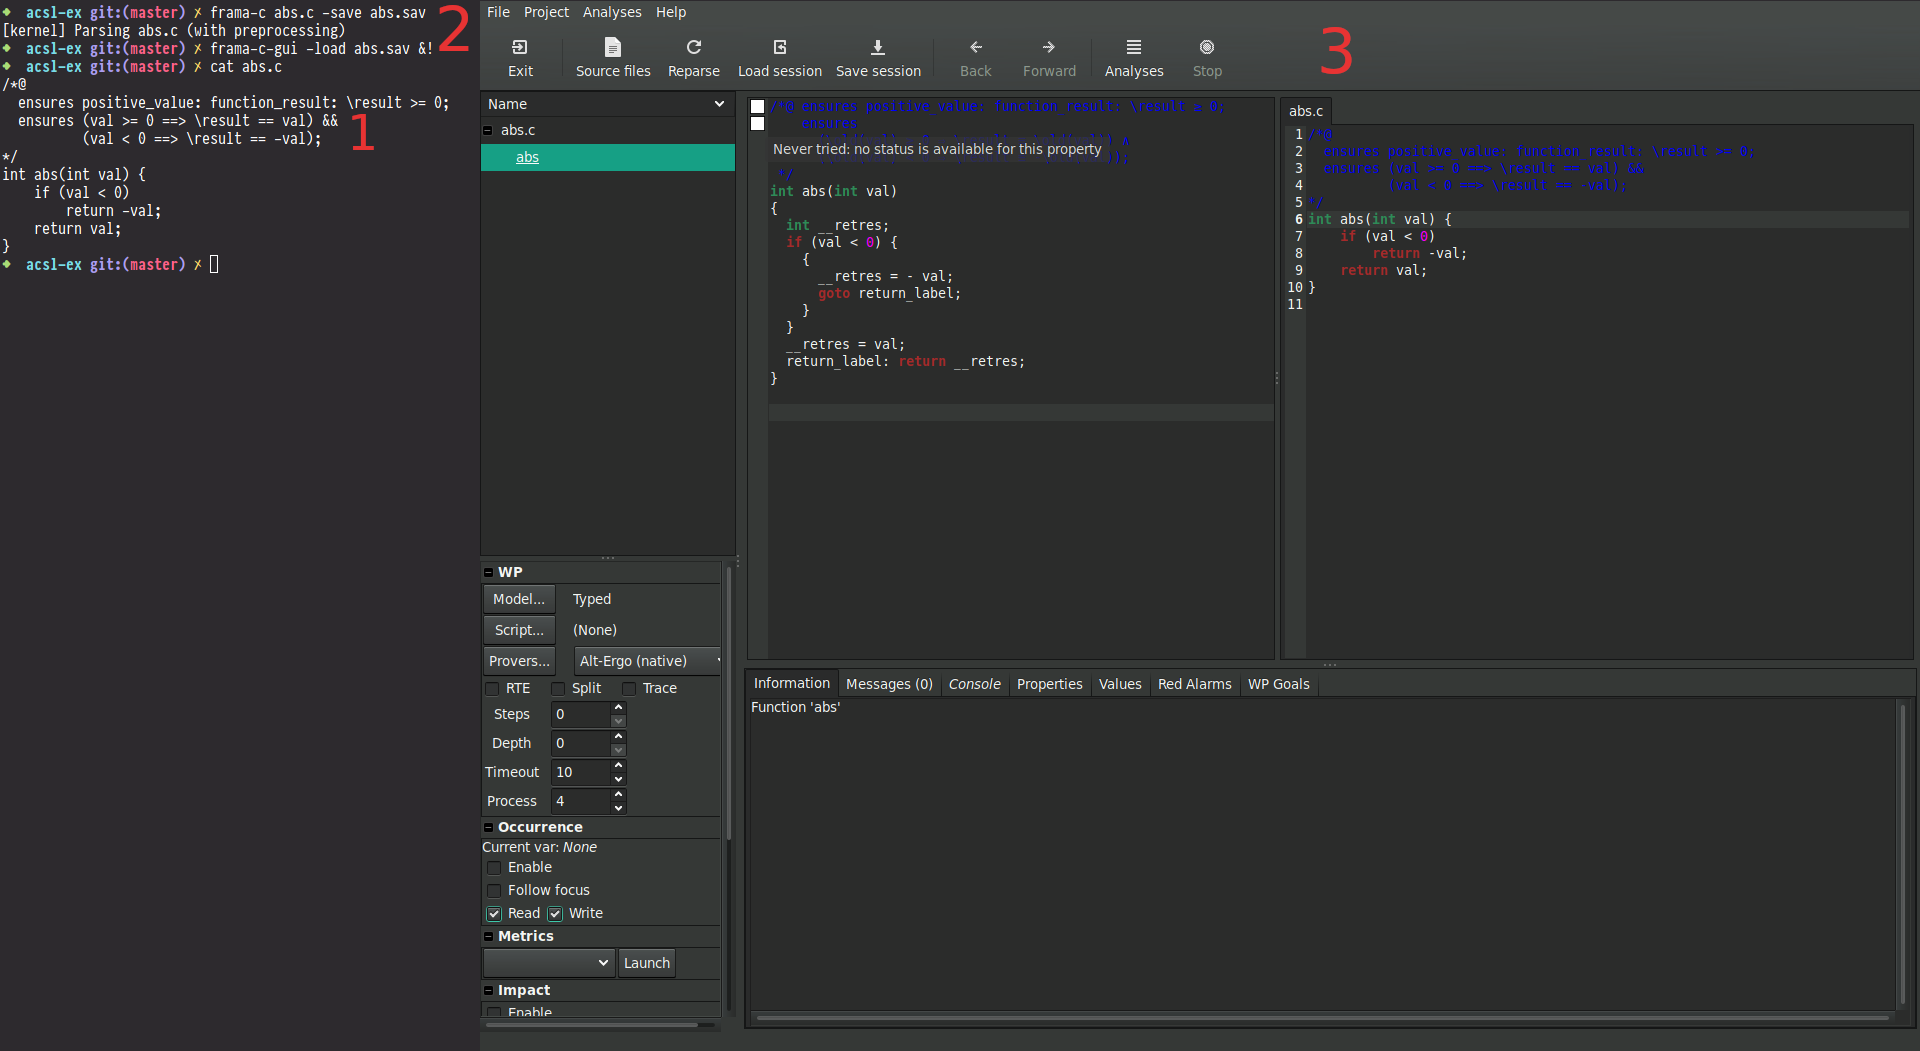
\includegraphics[width=1\textwidth]{img/exemplu}
  \caption{Exemplu \texttt{FramaC}: (1) adnotări, (2) CLI, (3) GUI}
  \label{fig:exframa}
\end{figure}

Deși poate fi utilizat în această formă, este recomandabil ca \texttt{FramaC} să fie
apelat folosind plugin-uri specifice. În verificarea proiectului \texttt{Monocypher},
vom folosi plugin-ul \texttt{Eva} (varianta actualizată [\emph{Evolved}] a
\emph{Value Analysis}), care este descris în secțiunea următoare.

Observăm, de asemenea, că în imaginea din \ref{fig:exframa}, în dreptul adnotărilor
apar pătrate goale, cu mesajul \texttt{Never tried. No status is available for %
  this property}. Aceasta se datorează faptului că nu s-a apelat niciun plugin,
iar uneltele de bază pentru verificare incluse doar în \texttt{frama-c} nu pot
verifica codul inclus. O verificare simplă poate fi rulată cu plugin-ul \texttt{RTE}
(\emph{RunTime Evaluation}), de exemplu, dar ne vom concentra în continuare
pe \texttt{Eva}.


%%%%%%%%%%%%%%%%%%%%%%%%%%%%%%%%%%%%%%%%%%%%%%%%%%%%%%%%%%%%%%%%%%%%%% 

\newpage
\section{\texttt{Eva}}

\subsection{Motivație}
\indent\indent Ca majoritatea uneltelor criptografice, \texttt{Monocypher}
se bazează pe expresii și operații numerice, eventual cu valori foarte
mari și prelucrări pe biți. Aceasta îl face să fie posibil vulnerabil
atît la operații matematice interzise (precum împărțirea la 0 sau depășirea
intervalului de valori permise de tipul de date folosit) sau la scurgeri de memorie.

\texttt{Eva} se bazează pe o teorie matematică numită \emph{interpretare abstractă}
(\cite{wikiabs}), conform și \cite{eva}, care îl face în special potrivit
pentru verificarea programelor cu conținut aritmetic bogat. De asemenea,
\texttt{Eva} poate detecta și scurgeri de memorie sau operații nepermise la nivel
de memorie alocată, dar pentru verificări mai avansate în special asupra memoriei,
este recomandabil să se folosească \texttt{Valgrind} (\cite{valgrind}).

%%%%%%%%%%%%%%%%%%%%%%%%%%%%%%%%%%%%%%%%%%%%%%%%%%%%%%%%%%%%%%%%%%%%%% 

\subsection{Interpretarea abstractă}

\indent\indent Această teorie matematică este folosită în semantica unor
programe, mai precis în aproximarea valorilor pe care le au variabilele în diverse
blocuri de cod. Într-un anume sens, interpretarea abstractă poate fi asemănată
cu execuția simbolică sau concolică, prin aceea că încearcă să folosească
bucățile de cod dimprejurul unor operații cu variabile pentru a aproxima
valorile pe care le au acele variabile. Însă, în forma simplă cel puțin,
interpretarea abstractă nu folosește SMT sau SAT solvere.

Un exemplu tipic care motivează și totodată introduce modul de lucru al
interpretării abstracte este următorul. Presupunem că la o petrecere sînt
invitate niște persoane și vrem să ne asigurăm că știm exact ce persoane au venit.
Varianta care funcționează sigur este să cerem fiecărei persoane să se identifice
cu un identificator unic, cum este CNP-ul în România. Atunci am avea o informație
precisă, nu aproximativă. Presupunem, însă, că această variantă nu este fezabilă,
deoarece CNP-ul cere prea mult spațiu de stocare, să spunem. Atunci putem folosi
doar numele participanților, fără spațiu suplimentar, deoarece oricum ei și-ar fi
dat numele. Dar atunci, nu mai putem spune cu exactitate dacă o anumită persoană
este prezentă. Atunci cînd există conflicte de nume, putem semnala o atenționare
sau, dacă situația este serioasă (e.g.\ căutăm pe lista invitaților persoana care
a spart candelabrul), chiar putem plasa o alarmă în dreptul tuturor celor care
au același nume sau diferă prin doar 1-2 litere, chiar cu riscul ca alarma să fie
falsă.

Ideea de bază este că se poate da o semantică destul de precisă în cazul majorității
limbajelor de programare --- așa-numita \emph{semantică concretă} ---, care să țină
cont și de aspecte operaționale ale limbajului, i.e.\ implementarea propriu-zisă
plus compilatoarele. Dar, dacă este necesar să se evalueze un anumit program scris
în limbajul respectiv, chiar în prezența semanticii concrete sau operaționale,
nu se pot verifica precis valorile pe care le au toate variabilele din program
(o problemă imposibil de rezolvat, în general, din motive de calculabilitate).
Astfel că este necesar să se folosească aproximări, bazate pe diverse teorii,
cu riscul asumat de supra- sau sub-aproximare.

Ideea de bază în asemenea situații este să se \emph{abstractizeze}. Adică,
pornind de la semantica concretă, care este destul de precisă din punct de vedere
teoretic, dar aproape imposibil de folosit din punct de vedere practic,
se pot forma așa-numitele \emph{semantici abstracte}, în care interpretarea
programelor este dată într-un anumit cadru matematic. Detalii și exemple se pot
găsi pe site-ul lui Patrick Cousot, cel care a introdus metoda interpretării abstracte
în anul 1970, împreună cu Radhia Cousot (\cite{abs}).

Interpretarea abstractă poate fi făcută \emph{ad-hoc}, pentru un anumit program
sau fragment. Prezentăm un exemplu, preluat de la \cite{wikiabs}. Presupunem că
avem o mulțime de numere întregi și vrem să le \qq{abstractizăm} către o mulțime
de semne $ +, -, 0 $, pentru eficiența stocării.

Fie $ L $ mulțimea concretă, adică aceea a numerelor întregi pe care vrem să le
abstractizăm și fie $ L' $ mulțimea abstractă, pe care vrem să o construim.
Cea mai simplă metodă de a face trecerea de la $ L $ la $ L' $ este să folosim
o funcție totală, care ar face corespondența clară. O astfel de funcție,
$ \alpha : L \to L' $ se va numi \emph{funcție de abstractizare}. Invers, o funcție
$ \gamma : L' \to L $ se va numi \emph{funcție de concretizare}.

Presupunem, în plus, că mulțimea $ L $ este și ordonată, o informație pe
care vrem să o păstrăm prin abstractizare. De aceea, trebuie să presupunem că
funcția $ \alpha $ este compatibilă cu ordinea, i.e. este crescătoare, adică
$ x \leq y $ în $ L $ implică $ \alpha(x) \leq \alpha(y) $ în $ L' $.

Mai general, putem fi interesați și de corespondența abstract-concret pentru bucăți
de program, deci putem dori funcții definite doar pe submulțimi ale lui $ L $.

Astfel, fie $ L_1, L_2, L'_1, L'_2 $ mulțimi ordonate și presupunem că semantica
concretă a mulțimii $ L_1 $ este dată de o funcție $ f : L_1 \to L_2 $. O funcție
$ f' : L_1' \to L'_2 $ se numește \emph{abstracție validă} a lui $ f $ dacă
este compatibilă atît cu abstractizarea, cît și cu concretizarea, adică are loc:
\[
  (f \circ \gamma)(x') \leq (\gamma \circ f')(x'), \quad \forall x' \in L'_1.
\]

\begin{figure}[!htbp]
  \centering
    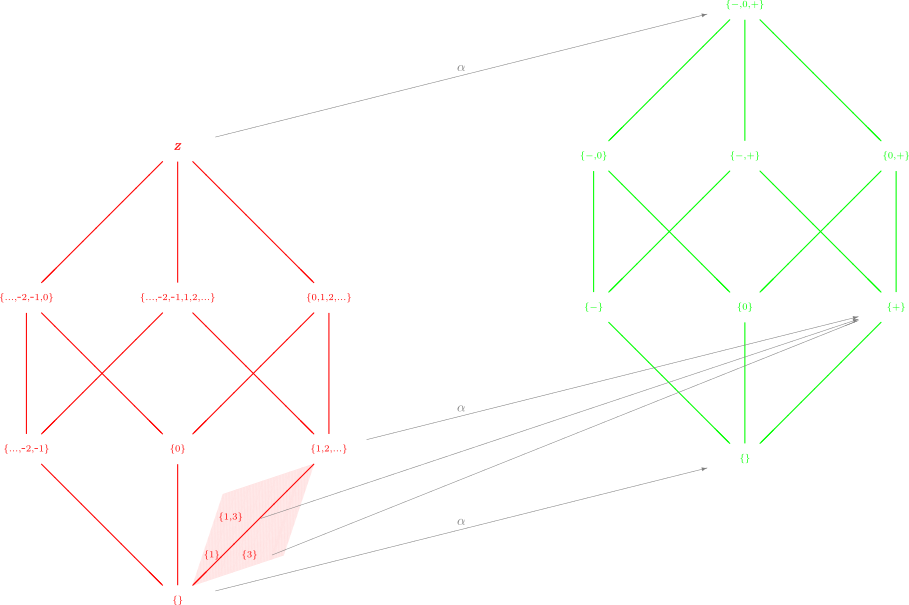
\includegraphics[width=1\textwidth]{img/abs}
    \caption{\textit{Abstractizarea unei (sub)mulțimi de întregi} (\cite{wikiabs})}
\end{figure}

În funcție de structura pe care o au mulțimile $ L_1, L_2, L'_1, L'_2 $ (de exemplu,
de latice cu proprietăți suplimentare, cel mai adesea), funcțiile $ f, f' $,
dar și elementele care să satisfacă inegalitatea de mai sus pot fi mai greu sau mai
ușor de găsit.

Se poate arăta că există un \emph{operator de lărgire} $ \nabla $ care poate satisface
relația de mai sus, însă cu prețul considerării unei mulțimi mai mare, caz în care
se realizează \emph{supra-aproximarea} sau, în ipoteza existenței unei
\emph{conexiuni Galois} între mulțimile parțial ordonate luate în discuție,
se poate realiza o sub-aproximare.

\vspace{1cm}

Revenind la \texttt{Eva}, programul are la bază implementări ale interpretării
abstracte, astfel că este folosit pentru a urmări valorile unor variabile.
În cazul \texttt{Monocypher}, \texttt{Eva} se va dovedi util din cel puțin două
privințe:
\begin{itemize}
\item pe de o parte, poate să raporteze dacă există neterminare, caz în care
  prelucrările numerice din algoritmi sînt greșite, cel puțin pe un caz;
\item poate să raporteze dacă valorile numerice folosite ies din marja tipurilor de
  date folosite (\emph{overflow}), situație care este de asemenea de interes, cu atît
  mai mult cu cît programul pune accent pe eficiență și viteză, iar algoritmii de
  criptare folosiți lucrează cu tipuri de date mici.
\end{itemize}




%%% Local Variables:
%%% mode: latex
%%% TeX-master: "../mono-frama"
%%% End:
